% $Id$ %
\chapter{\label{ref:rockbox_interface}The Rockbox interface}
\section{Your \dap}
\begin{center}
  \opt{player}{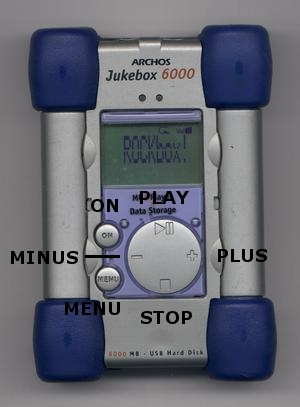
\includegraphics[height=11.8cm]{rockbox_interface/images/player-front.png}}
  \opt{recorder,recorderv2fm}{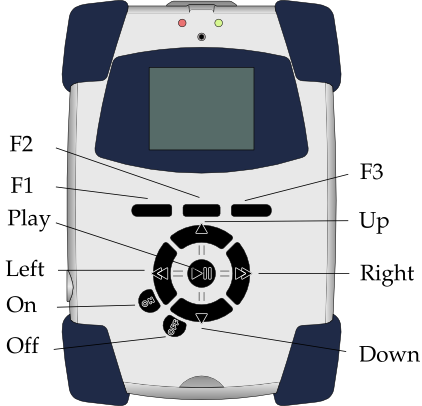
\includegraphics[height=11.8cm]{rockbox_interface/images/recorderv2fm-front.png}}
  \opt{ondio}{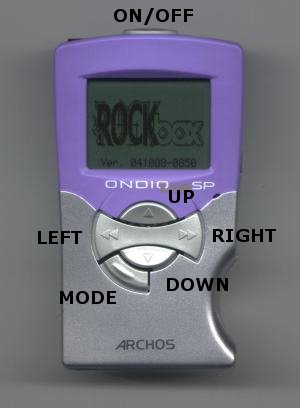
\includegraphics[height=11.8cm]{rockbox_interface/images/ondio-front.png}}
  \opt{h1xx}{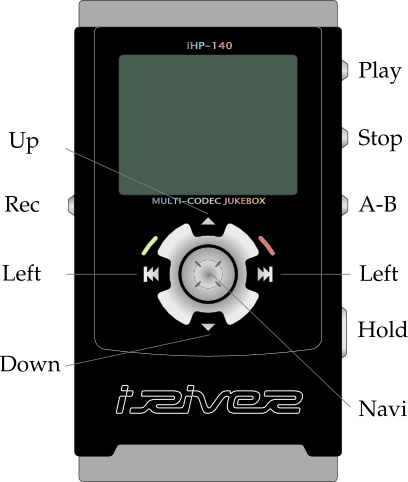
\includegraphics[height=11.8cm]{rockbox_interface/images/h1xx-front.png}}
  \opt{h300}{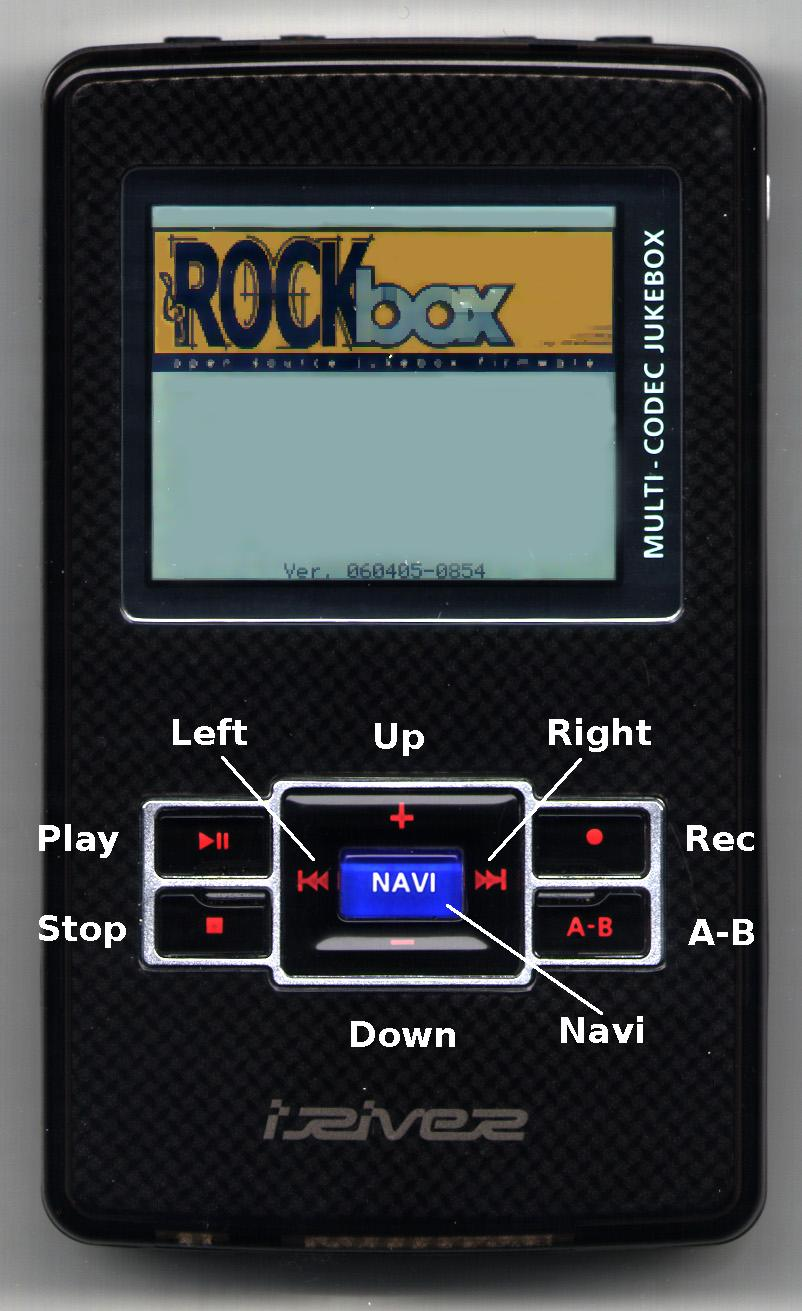
\includegraphics[height=11.8cm]{rockbox_interface/images/h300-front.jpg}}
\end{center}

Throughout this manual, the buttons on the \dap\ are labelled according to the
picture above. To turn on and shut down your \dap, the following keys are used:

\begin{table}
    \begin{btnmap}{}{}
      \opt{IRIVER_H100_PAD,IRIVER_H300_PAD}{\ButtonOn}
      \opt{IPOD_4G_PAD}{\ButtonMenu\ or \ButtonSelect}
      \opt{ONDIO_PAD}{\ButtonOff}\opt{RECORDER_PAD,PLAYER_PAD}
        {Hold \ButtonOn\ for 2{}-3s}
      \opt{IAUDIO_X5_PAD}{\ButtonPower} 
      & Start Rockbox\\
      \opt{IRIVER_H100_PAD,IRIVER_H300_PAD}{Hold \ButtonOff}
      \opt{IPOD_4G_PAD}{Hold \ButtonPlay}
      \opt{ONDIO_PAD,recorderv2fm}{Hold \ButtonOff}
      \opt{recorder}{Double tap \ButtonOff\ when playback is stopped}
      \opt{PLAYER_PAD}{From the Main Menu, select \textbf{Shutdown}}
      \opt{IAUDIO_X5_PAD}{Hold \ButtonPower}
      & Shutdown Rockbox\\
    \end{btnmap}
\end{table}
\label{ref:Safeshutdown}On shutdown, Rockbox automatically saves its settings.

\opt{PLAYER_PAD,RECORDER_PAD,ONDIO_PAD}{
  In the unlikely event of a software failure, a hardware power off can be
  performed by holding down 
  \opt{PLAYER_PAD}{\ButtonStop}
  \opt{RECORDER_PAD,ONDIO_PAD}{\ButtonOff}
  until the Jukebox power light goes off.
}

\section{\label{ref:file_browser}File Browser}
\screenshot{rockbox_interface/images/ss-file-browser}{The file browser}{}
Rockbox lets you browse your music in either of two ways. The 
\setting{File Browser} lets you navigate through the files and folders on 
your \dap, entering folders and executing the default action on each file.
To help differentiate files, each file format is displayed with an icon. 

The \setting{Tag Cache Browser}, on the other hand, allows you to navigate 
through the music on your player using categories like album, artist, genre, etc.  

You can select whether to browse using the \setting{File Browser} or the 
\setting{Tag Cache Browser} by adjusting the \setting{Show Files} setting.  
If you choose the \setting{File Browser}, the \setting{Show Files} setting also 
lets you select what types of files you wish to view.  See page 
\pageref{ref:ShowFiles} for more information on the \setting{Show Files} setting.

\note{The \setting{File Browser} allows you to manipulate your files in ways that 
are not available within the \setting{Tag Cache Browser}.  Read more about 
\setting{Tag Cache} in Section \ref{ref:tagcache}.  The remainder of this section
deals with the \setting{File Browser}.}

\subsection{\label{ref:controls}File Browser Controls}
\begin{table}
    \begin{btnmap}{}{}
      \opt{IRIVER_H100_PAD,IRIVER_H300_PAD,ONDIO_PAD,RECORDER_PAD,IAUDIO_X5_PAD}
        {\ButtonUp/\ButtonDown}
      \opt{PLAYER_PAD}{\ButtonLeft/\ButtonRight}
      \opt{IPOD_4G_PAD}{\ButtonScrollBack/\ButtonScrollFwd} 
         & Go to previous/next item in list. If you are on the first/last 
           entry, the cursor will wrap to the last/first entry.\\
      %
      \opt{IRIVER_H100_PAD,IRIVER_H300_PAD,RECORDER_PAD}
        {\ButtonOn+\ButtonUp/\ButtonDown}
      \opt{PLAYER_PAD,IPOD_4G_PAD,IAUDIO_X5_PAD}{n/a}
      \opt{ONDIO_PAD}{n/a}
      & Move one page up/down on the list.\\
      %
      \opt{IRIVER_H100_PAD,IRIVER_H300_PAD,RECORDER_PAD,IAUDIO_X5_PAD,ONDIO_PAD,IPOD_4G_PAD}{\ButtonLeft}
      \opt{PLAYER_PAD}{\ButtonStop} 
      & Go to the parent directory. \\
      %
      \opt{IRIVER_H100_PAD,IRIVER_H300_PAD,IAUDIO_X5_PAD,IPOD_4G_PAD}
        {\ButtonRight/\ButtonSelect}
      \opt{PLAYER_PAD}{\ButtonPlay}
      \opt{ONDIO_PAD}{\ButtonRight}
      \opt{RECORDER_PAD}{\ButtonRight/\ButtonPlay}
      & Executes an action. Depending on the file type, that action may vary.
        (See page \pageref{ref:Filemenu}) \\
      %
      \opt{IRIVER_H100_PAD,IRIVER_H300_PAD,PLAYER_PAD,RECORDER_PAD}{\ButtonOn}
      \opt{IAUDIO_X5_PAD,IPOD_4G_PAD}{\ButtonPlay}
      \opt{ONDIO_PAD}{Short press on \ButtonMenu} 
      & If there is a MP3 playing, returns to the While Playing Screen (WPS)
        without stopping playback.  \\
      %
      \opt{IRIVER_H100_PAD,IRIVER_H300_PAD,IAUDIO_X5_PAD,IPOD_4G_PAD}
        {Hold \ButtonSelect}
      \opt{RECORDER_PAD,PLAYER_PAD}{Hold \ButtonPlay/\ButtonOn+\ButtonPlay}
      \opt{ONDIO_PAD}{Hold \ButtonRight} 
      & Enter the File Menu\\
      %
      \opt{IRIVER_H100_PAD,IRIVER_H300_PAD}{\ButtonMode}
      \opt{RECORDER_PAD}{\ButtonFOne}
      \opt{PLAYER_PAD,IPOD_4G_PAD,ONDIO_PAD,IPOD_VIDEO_PAD}{\ButtonMenu}
      \opt{IAUDIO_X5_PAD}{Press \ButtonRec}
      & Enter the Main Menu \\
      %
      \opt{RECORDER_PAD}{
        \ButtonFTwo & Switches to the Browse/Play Quick Menu \\
        %
        \ButtonFThree & Switches to the Display Quick Menu \\ 
        %
      }
    \end{btnmap}
\end{table}

\opt{RECORDER_PAD}{
  The functions of the F keys are also summarised on the button bar at the
  bottom of the screen.
}

\subsection{\label{ref:Filemenu}\label{ref:PartIISectionFM}File Menu}
\screenshot{rockbox_interface/images/ss-file-menu}{The File Menu}{}

The \setting{File Menu} allows you to perform certain operations on files or 
folders.  To access the \setting{File Menu}, position the selector over a file 
or folder and 
	\opt{IRIVER_H100_PAD,IRIVER_H300_PAD,IAUDIO_X5_PAD,IPOD_4G_PAD}
		{hold the \ButtonSelect\ button.}
	\opt{RECORDER_PAD,PLAYER_PAD}{press the \ButtonPlay/\ButtonOn+\ButtonPlay\ 
	  buttons.}
  \opt{ONDIO_PAD}{hold the \ButtonRight\ button.}
  
\note{The \setting{File Menu} is a context sensitive menu.  If the 
\setting{File Menu} is invoked on a file, it will display options available 
for files.  If the \setting{File Menu} is invoked on a folder or directory, 
it will display options for directories.}

The \setting{File Menu} contains the following options (unless otherwise noted, 
each option pertains both to files and directories):

\begin{description}
\item [Playlist:]
  Enters the \setting{Playlist Submenu} (see below).
\item [Rename:]
  This function lets the user modify a file name.
\item [Cut:]
  Copies the name of the currently selected file or directory to the clipboard
  and marks it to be 'cut'.
\item [Copy:]
  Copies the name of the currently selected file or directory to the clipboard
  and marks it to be 'copied'.
\item [Paste:]
  Only visible if a file or directory name is on the clipboard. When selected
  it will move or copy the clipboard to the current directory.
\item [Delete:]
  Deletes the currently selected file.  This option applies only to files, and
  not to directories.  Rockbox will ask for confirmation before deleting a file.
  Press
  	\opt{IRIVER_H100_PAD,IRIVER_H300_PAD,IAUDIO_X5_PAD,IPOD_4G_PAD,IPOD_VIDEO_PAD}
      {\ButtonSelect}
    \opt{PLAYER_PAD,RECORDER_PAD}{\ButtonPlay}
    \opt{ONDIO_PAD}{\ButtonRight}
 to confirm deletion or any other key to cancel.
\item [Delete Directory:]
  Deletes the currently selected directory and all of the files and folders
  contained in the selected directory.  Deleted directories cannot be recovered.
  Use this feature with caution!
\item [Open with:] 
  Runs a viewer plugin on the file. Normally, when a file is selected in Rockbox,
  Rockbox automatically detects the file type and runs the appropriate plugin.
  The \setting{Open With} function can be used to override the default action and
  select a viewer by hand.  For example, this function can be used to view a text file
  even if the file has a non-standard extension (i.e., the file has an extension
  of something other than ``.txt'').  See page \textmd{\pageref{ref:Viewersplugins}} 
  for more details on viewers.
\item [Create Directory:]
  Makes a new folder in the current folder on the disk.
\end{description}

\subsection{\label{ref:Playlistsubmenu}Playlist Submenu}
\screenshot{rockbox_interface/images/ss-playlist-menu}{The Playlist Submenu}{}
The \setting{Playlist Submenu} allows you to put tracks into a ``dynamic playlist''.
If there is no music currently playing, Rockbox will create a new dynamic playlist
and put the selected track(s) into the playlist.  If there is music currently playing,
Rockbox will put the selected track(s) into the current playlist.  The place in which
the newly selected tracks are added to the playlist is determined by the following
options:

\begin{description}
\item [Insert:]
  Add track(s) to playlist. If no other tracks have been inserted then the
  selected track will be added immediately after current playing track,
  otherwise they will be added to end of insertion list.
\item [Insert next:] 
  Add track(s) immediately after current playing track, no matter what else has
  been inserted.
\item [Insert last:]
  Add track(s) to end of playlist.
\item [Queue:]
  Queue is the same as Insert except queued tracks are deleted immediately from
  the playlist after they've been played. Also, queued tracks are not saved to
  the playlist file (see page \pageref{ref:playlistoptions}).
\item [Queue next:]
  Queue track(s) immediately after current playing track.
\item [Queue last:]
  Queue track(s) at end of playlist.
\end{description}

The \setting{Playlist Submenu} can be used to add either single tracks or 
entire directories to a playlist. If the \setting{Playlist Submenu} is 
invoked on a single track, it will put only that track into the playlist.  
On the other hand, if the \setting{Playlist Submenu} is invoked on a 
directory, Rockbox adds all of the tracks in that directory to the playlist.  

\note{You can control whether or not Rockbox includes the contents of subdirectories
when adding an entire directory to a playlists.  Set the \setting{Main Menu 
$\rightarrow$ Playlist Options $\rightarrow$ Recusively Insert Directories} setting to 
\setting{Yes} if you would like Rockbox to include tracks in subdirectories as well as tracks
in the currently-selected directory.}

If you want to have Rockbox create a playlist of a whole folder (to play an entire 
album, for example), use the \setting{File Browser} to select the song. When a single 
song is selected from the \setting{File Browser}, Rockbox will automatically create a 
playlist with all songs in the current folder. However, if you want to play only a single 
song and then stop, stop playback, navigate to the song you want to play, and use the 
\setting{Playlist $\rightarrow$ Insert} function to select the song.

Dynamic playlists are saved so resume will restore them exactly as they were before
shutdown.

\note{To view, save or reshuffle the current dynamic playlist, use the 
\setting{Playlist Options} setting in the WPS Context Menu.}

\subsection{Virtual Keyboard}
\screenshot{rockbox_interface/images/ss-virtual-keyboard}{The virtual keyboard}{}
This is the virtual keyboard that is used when entering file names in Rockbox.

\opt{IRIVER_H100_PAD,IRIVER_H300_PAD,IAUDIO_X5_PAD,RECORDER_PAD}{
    \begin{table}
    \begin{btnmap}{}{}
      \opt{IRIVER_H100_PAD,IRIVER_H300_PAD,IAUDIO_X5_PAD,RECORDER_PAD}
        {\ButtonUp/\ButtonDown\\ButtonLeft/\ButtonRight}
      & Move about the virtual keyboard (moves the solid cursor) \\
      %
      \opt{IRIVER_H100_PAD,IRIVER_H300_PAD,RECORDER_PAD}
        {\ButtonOn+\ButtonLeft/\ButtonRight}
      \opt{IAUDIO_X5_PAD}{Please add correct keys} 
      & Move about within the current file name (moves the line cursor) \\
      %
      \opt{IRIVER_H100_PAD,IRIVER_H300_PAD}{\ButtonSelect}
      \opt{RECORDER_PAD}{\ButtonPlay}
      \opt{IAUDIO_X5_PAD}{Please add correct keys} 
      & Inserts the currently selected keyboard letter at the current
        filename cursor position \\
      %
      \opt{IRIVER_H100_PAD,IRIVER_H300_PAD,RECORDER_PAD}{\ButtonOff}
      \opt{IAUDIO_X5_PAD}{Please add correct keys} 
      & Exits the virtual keyboard without saving any changes \\
      %
      \opt{IRIVER_H100_PAD,IRIVER_H300_PAD,IAUDIO_X5_PAD}{n/a}
      \opt{RECORDER_PAD}{\ButtonFOne}
      & SHIFT: Shifts between the upper case, lower case and accented keyboards \\
      %
      \opt{IRIVER_H100_PAD,IRIVER_H300_PAD}{\ButtonOn}
      \opt{RECORDER_PAD}{\ButtonFTwo}
      \opt{IAUDIO_X5_PAD}{Please add correct keys} 
      & OK: Exits the virtual keyboard and saves any changes \\
      %
      \opt{IRIVER_H100_PAD,IRIVER_H300_PAD}{\ButtonRec}
      \opt{RECORDER_PAD}{\ButtonFThree}
      \opt{IAUDIO_X5_PAD}{Please add correct keys} 
      & DEL: Deletes the character before the current filename cursor \\
      %
      \opt{SWCODEC}{
        \opt{IRIVER_H100_PAD,IRIVER_H300_PAD}{\ButtonOn+\ButtonMode}
        \opt{IAUDIO_X5_PAD}{Please add correct keys} 
        & Enters Morse input mode\\
      }
    \end{btnmap}
  \end{table}
}

\opt{IPOD_4G_PAD}{
  \textbf{Picker area}
  \begin{table}
    \begin{btnmap}{}{}
      \ButtonScrollFwd/\ButtonScrollBack & Move about the virtual keyboard \\
      \ButtonLeft/\ButtonRight		 & (moves the solid cursor).
          If you move out of the picker area with \ButtonScrollFwd/\ButtonScrollBack,
          you get to the line edit mode. \\
      \ButtonSelect 
        & Inserts the currently selected keyboard letter at the current
          filename cursor position \\
      Hold \ButtonSelect
      	& OK: Exits the virtual keyboard and saves any changes \\
      \ButtonMenu
        & Exits the virtual keyboard without saving any changes\\
    \end{btnmap}
  \end{table}
  \textbf{Line edit mode}
  \begin{table}
    \begin{btnmap}{}{}
      \ButtonLeft/\ButtonRight & Move left and right\\
      \ButtonSelect & Deletes the letter to the left of the cursor\\
      \ButtonScrollFwd/\ButtonScrollBack & Returns to the picker area\\
    \end{btnmap}
  \end{table}
}
\opt{ondio}{
  \textbf{Picker area}
  \begin{table}
    \begin{btnmap}{}{}
      \ButtonUp/\ButtonDown/\ButtonLeft/\ButtonRight
        & Move about the virtual keyboard (moves the solid cursor).
          If you move out of the picker area with \ButtonUp/\ButtonDown,
          you get to the line edit mode. \\
      \ButtonMenu 
        & Selects the letter underneath the cursor. \\
      Long press on \ButtonMenu 
       & Accepts the currently selected letter\\
      \ButtonOff 
       & Aborts the currently selected letter\\
    \end{btnmap}
  \end{table}
  \textbf{Line edit mode}
  \begin{table}
    \begin{btnmap}{}{}
      \ButtonLeft/\ButtonRight & Move left and right\\
      \ButtonMenu & Deletes the letter to the left of the cursor\\
      Long press on \ButtonMenu & Accepts the deletion\\
      \ButtonUp/\ButtonDown & Returns to the picker area\\
    \end{btnmap}
  \end{table}
}\opt{player}{
  The current filename is always listed on the first line of the display. The
  second line of the display can contain the character selection bar, as in the
  screenshot above, or  one of a number of other options.
  \begin{table}
    \begin{btnmap}{}{}
      \ButtonLeft/\ButtonRight & Moves the arrow to/from the filename \\
                               & and changes between the character bar \\
                               & and BACKSPACE, DELETE, ACCEPT and ABORT. \\
      \ButtonPlay/\ButtonStop & Varies (see below) \\
      \ButtonMenu & Shift.  When the character selection bar is selected\\
                  & this changes between upper case, lower case, \\
                  & and accented letters. \\
    \end{btnmap}
  \end{table}

  The function of the \ButtonPlay\ and \ButtonStop\ buttons depends on what the
  arrow is pointing to, as follows.
  
  \begin{table}
      \begin{center}
      \begin{tabularx}{.75\textwidth}{lX}
        \textbf{Selected option} & \textbf{Play/Stop function} \\\midrule
        filename & Moves the cursor left (\ButtonStop) \\
                 & or right (\ButtonPlay) within the filename \\
        character bar & Moves the character bar to the next (\ButtonPlay)\\
                      & or previous (\ButtonStop) character. \\
        BACKSPACE & \ButtonPlay deletes the character before \\
                  & the current cursor position \\
        DELETE & \ButtonPlay deletes the character at the \\
               & current cursor position\\
        ACCEPT & \ButtonPlay exits the virtual keyboard and \\
               & saves any changes \\
        ABORT & \ButtonPlay exits the virtual keyboard and \\
              & discards any changes \\\bottomrule
      \end{tabularx}
    \end{center}
  \end{table}
}

% $Id$ %
\section{\label{ref:database}Database}

\subsection{Introduction}
This chapter describes the Rockbox music database system. Using the information
contained in the tags (ID3v1, ID3v2%
  \opt{swcodec}{, Vorbis Comments, Apev2, etc.}%
) in your audio files, Rockbox builds and maintains a database of the music
files on your player and allows you to browse them by Artist, Album, Genre, 
Song Name, etc.  The criteria the database uses to sort the songs can be completely
 customised. More information on how to achieve this can be found on the Rockbox
 website at \wikilink{DataBase}. 

\subsection{Initializing the Database}
The first time you use the database, Rockbox will scan your disk for audio files.
This can take quite a while depending on the number of files on your \dap{}.
This scan happens in the background, so you can choose to return to the
Main Menu and continue to listen to music.
If you shut down your player, the scan will continue next time you turn it on.
After the scan is finished you may be prompted to restart your \dap{} before
you can use the database.

\subsubsection{Ignoring Directories During Database Initialization}

You may have directories on your \dap{} whose contents should not be added
to the database. Placing a file named \fname{database.ignore} in a directory
will exclude the files in that directory and all its subdirectories from
scanning their tags and adding them to the database. This will speed up the
database initialization.

If a subdirectory of an 'ignored' directory should still be scanned, place a
file named \fname{database.unignore} in it. The files in that directory and
its subdirectories will be scanned and added to the database.

\subsection{\label{ref:databasemenu}The Database Menu}

\begin{description}
  \opt{swcodec}{
  \item[Load To RAM]
    The database can either be kept on disk (to save memory), or
    loaded into RAM (for fast browsing). Setting this to \setting{Yes} loads
    the database to RAM, allowing faster browsing and searching. Setting this
    option to \setting{No} keeps the database on the disk, meaning slower 
    browsing but it does not use extra RAM and saves some battery on boot up. 
    
    \note{If you browse your music frequently using the database, you should
      load to RAM, as this will reduce the overall battery consumption because
      the disk will not need to spin on each search.}
  }
  
\item[Auto Update]
  If \setting{Auto update} is set to \setting{on}, each time the \dap{}
  boots, the database will automatically be updated.
  \opt{swcodec}{
    \note{The \setting{Auto Update} will only check for deleted files if the
      \setting{Directory Cache} (\setting{Settings $\rightarrow$ General
      Settings $\rightarrow$ System $\rightarrow$ Disk $\rightarrow$
      Directory Cache}) is enabled. \setting{Update now} includes that check
      whether dircache has been enabled or not.}
  }%

\item[Initialize Now]
  You can force Rockbox to rescan your disk for tagged files by
  using the \setting{Initialize Now} function in the \setting{Database
    Menu}.
  \warn{\setting{Initialize Now} removes all database files (removing
    runtimedb data also) and rebuilds the database from scratch.}

\item[Update Now]
  \setting{Update now} causes the database to detect new and deleted files
  \opt{swcodec}{
    \note{Unlike the \setting{Auto Update} function, \setting{Update Now}
      will update the database regardless of whether the \setting{Directory Cache}
      is enabled. Thus, an update using \setting{Update now} may take a long
      time.
    }
  }
  Unlike \setting{Initialize Now}, the \setting{Update Now} function
  does not remove runtime database information.
  
\item[Gather Runtime Data]
  When enabled, rockbox will record how often and how long a track is being played, 
  when it was last played and its rating. This information can be displayed in
  the WPS and is used in the database browser to, for example, show the most played, 
  unplayed and most recently played tracks.
  
\item[Export Modifications]
  This allows for the runtime data to be exported to the file \\
  \fname{/.rockbox/database\_changelog.txt}, which backs up the runtime data in
  ASCII format. This is needed when database structures change, because new
  code cannot read old database code. But, all modifications
  exported to ASCII format should be readable by all database versions.
  
\item[Import Modifications.]
  Allows the \fname{/.rockbox/database\_changelog.txt} backup to be 
  conveniently loaded into the database. If \setting{Auto Update} is
  enabled this is performed automatically when the database is initialized.
  
\end{description}

\subsection{Using the Database}
Once the database has been initialized, you can browse your music 
by Artist, Album, Genre, Song Name, etc.  To use the database, go to the
 \setting{Main Menu} and select \setting{Database}.\\

\note{You may need to increase the value of the \setting{Max files in dir 
browser} setting (\setting{Settings $\rightarrow$ General Settings
$\rightarrow$ System $\rightarrow$ Limits}) in order to view long lists of
tracks in the ID3 database browser.\\

There is no option to turn off database completely. If you do not want
to use it just do not do the initial build of the database and do not load it
to RAM.}%

\begin{table}
\begin{center}
  \begin{tabularx}{.75\textwidth}{XXX}%
  \toprule%
  \textbf{Tag}   & \textbf{Type}  & \textbf{Origin} \\
  \midrule
  filename              & string    & system \\ 
  album                 & string    & id tag \\
  albumartist           & string    & id tag \\
  artist                & string    & id tag \\
  comment               & string    & id tag \\
  composer              & string    & id tag \\
  genre                 & string    & id tag \\
  grouping              & string    & id tag \\
  title                 & string    & id tag \\
  bitrate               & numeric   & id tag \\
  discnum               & numeric   & id tag \\
  year                  & numeric   & id tag \\
  tracknum              & numeric   & id tag/filename \\
  autoscore             & numeric   & runtime db \\
  lastplayed            & numeric   & runtime db \\
  playcount             & numeric   & runtime db \\
  Pm (play time - min)  & numeric   & runtime db \\
  Ps (play time - sec)  & numeric   & runtime db \\
  rating                & numeric   & runtime db \\
  commitid              & numeric   & system \\
  entryage              & numeric   & system \\
  length                & numeric   & system \\
  Lm (track len - min)  & numeric   & system \\
  Ls (track len - sec)  & numeric   & system \\
  \bottomrule
  \end{tabularx}
\end{center}
\end{table}

% $Id$ %
\section{\label{ref:WPS}While Playing Screen}
The While Playing Screen (WPS) displays various pieces of information about the
currently playing audio file.
%
\opt{lcd_bitmap}{%
  The appearance of the WPS can be configured using WPS configuration files.
  The items shown depend on your configuration -- all items can be turned on
  or off independently. Refer to \reference{ref:wps_tags} for details on how
  to change the display of the WPS.
  \begin{itemize}
    \nopt{ondio}{
    \item Status bar: The Status bar shows Battery level, charger status, 
      volume, play mode, repeat mode, shuffle mode\opt{rtc}{ and clock}.
      In contrast to all other items, the status bar is always at the top of
      the screen.
    }
    \opt{ondio}{
    \item Status bar: The Status bar shows Battery level, USB power mode, key
      lock status, memory access indicator. In contrast to all other items, the
      status bar is always at the top of the screen.
    }
  \item (Scrolling) path and filename of the current song.
  \item The ID3 track name.
  \item The ID3 album name.
  \item The ID3 artist name.
  \item Bit rate. VBR files display average bitrate and ``(avg)''
  \item Elapsed and total time.
  \item A slidebar progress meter representing where in the song you are.
  \item Peak meter.
  \end{itemize}
}
\opt{recorder,recorderv2fm,ondio}{
  \note{
  \begin{itemize}
  \item The number of lines shown depends on the size of the font used.
  \item The peak meter is only visible if you turn off the status bar or if
    using a small font that gives 8 or more display lines.
  \end{itemize}
  }
}
%
\opt{player}{
  \note{
  \begin{itemize}
  \item Playlist index/Playlist size: Artist {}- Title.
  \item Current{}-time Progress{}-indicator Left.
  \end{itemize}
  }
}

See \reference{ref:ConfiguringtheWPS} for details of customising
your WPS (While Playing Screen).


\subsection{\label{ref:WPS_Key_Controls}WPS Key Controls}

\begin{table}
  \begin{btnmap}{}{}
      \ActionWpsVolUp{} / \ActionWpsVolDown
      \opt{HAVEREMOTEKEYMAP}{& \ActionRCWpsVolUp{} / \ActionRCWpsVolDown}
      & Volume up/down.\\
      %
      \ActionWpsSkipPrev
       \opt{HAVEREMOTEKEYMAP}{& \ActionRCWpsSkipPrev}
      & Go to beginning of track, or if pressed while in the
        first seconds of a track, go to previous track.\\
      %
      \ActionWpsSeekBack
      \opt{HAVEREMOTEKEYMAP}{& \ActionRCWpsSeekBack}
      & Rewind in track.\\
      %
      \ActionWpsSkipNext
      \opt{HAVEREMOTEKEYMAP}{& \ActionRCWpsSkipNext}
      & Go to next track.\\
      %
      \ActionWpsSeekFwd
      \opt{HAVEREMOTEKEYMAP}{& \ActionRCWpsSeekFwd}
      & Fast forward in track.\\
      %
      \ActionWpsPlay
      \opt{HAVEREMOTEKEYMAP}{& \ActionRCWpsPlay}
      & Toggle play/pause.\\
      %
      \ActionWpsStop 
      \opt{HAVEREMOTEKEYMAP}{& \ActionRCWpsStop}
      & Stop playback.\\
      %
      \ActionWpsBrowse
      \opt{HAVEREMOTEKEYMAP}{& \ActionRCWpsBrowse}
      & Return to the \setting{File Browser}.\\
      %
      \ActionWpsContext
      \opt{HAVEREMOTEKEYMAP}{& \ActionRCWpsContext}
      & Enter \setting{WPS Context Menu}.\\
      %
      \opt{ONDIO_PAD}{\ActionWpsContext{} twice}%
      \nopt{ONDIO_PAD}{\ActionWpsMenu}%
      \opt{HAVEREMOTEKEYMAP}{& \ActionRCWpsMenu}
      & Enter \setting{Main Menu}%
      \opt{ONDIO_PAD}{ via the \setting{WPS Context Menu}}.\\%
      %
      \opt{quickscreen}{%
        \ActionWpsQuickScreen
        \opt{HAVEREMOTEKEYMAP}{& \ActionRCWpsQuickScreen}
          & Switches to the \setting{Quick Screen}.
          (see \reference{ref:QuickScreen}) \\}%
      %
      % software hold targets (currently Archos only)
      \nopt{hold_button}{%
          \opt{RECORDER_PAD}{\ButtonFOne+\ButtonDown}
          \opt{PLAYER_PAD}{\ButtonMenu+\ButtonStop}
          \opt{ONDIO_PAD}{\ButtonMenu+\ButtonDown}
          & Key lock on/off.\\
      }%
      %These actions need definitions for the other targets
      \opt{RECORDER_PAD}{%
        \ButtonFThree & Toggles Display quick screen.\\%
        \ButtonFOne+\ButtonPlay & Mute on/off.\\%
      }%
      \opt{PLAYER_PAD}{%
        \ButtonMenu+\ButtonPlay & Mute on/off.\\%
      }%
      % We explicitly list all the appropriate targets here and do no condition
      % on the 'pitchscreen' feature since some players have the feature but do
      % not have the button to go from the WPS to the pitch screen.
      \opt{RECORDER_PAD,IRIVER_H100_PAD,IRIVER_H300_PAD,IRIVER_H10_PAD,MROBE100_PAD%
	           ,GIGABEAT_PAD,GIGABEAT_S_PAD,SANSA_E200_PAD,SANSA_C200_PAD}{%
        \ActionWpsPitchScreen
        \opt{HAVEREMOTEKEYMAP}{& \ActionRCWpsPitchScreen}
         & Show \setting{Pitch Screen} (see \reference{sec:pitchscreen}).\\%
      }%
      \opt{PLAYER_PAD,RECORDER_PAD,IRIVER_H100_PAD,IRIVER_H300_PAD,IRIVER_H10_PAD%
          ,MROBE100_PAD,GIGABEAT_PAD,GIGABEAT_S_PAD,SANSA_E200_PAD,SANSA_C200_PAD}{%
        \ActionWpsIdThreeScreen 
          \opt{HAVEREMOTEKEYMAP}{& \ActionRCWpsIdThreeScreen}
          & Enter \setting{ID3 Viewer}.\\%
      }%
      \opt{RECORDER_PAD,IRIVER_H100_PAD,IRIVER_H300_PAD,IRIVER_H10_PAD,MROBE100_PAD%
          ,GIGABEAT_PAD,GIGABEAT_S_PAD,SANSA_E200_PAD,SANSA_C200_PAD}{%
         \ActionWpsAbSetBNextDir{} or }%
         % not all targets have the above action defined but the one below works on all
      Short \ActionWpsSkipNext{} + Long \ActionWpsSkipNext
      \opt{HAVEREMOTEKEYMAP}{
        &
          \opt{IRIVER_RC_H100_PAD}{\ActionRCWpsAbSetBNextDir{} or}
        Short \ActionRCWpsSkipNext{} + Long \ActionRCWpsSkipNext}
      & Skip to the next directory.\\
      %
      \opt{RECORDER_PAD,IRIVER_H100_PAD,IRIVER_H300_PAD,IRIVER_H10_PAD%
         ,MROBE100_PAD,GIGABEAT_PAD,GIGABEAT_S_PAD,SANSA_E200_PAD,SANSA_C200_PAD}{%
         \ActionWpsAbSetAPrevDir{} or }%
      Short \ActionWpsSkipPrev{} + Long \ActionWpsSkipPrev
      \opt{HAVEREMOTEKEYMAP}{
        &
          \opt{IRIVER_RC_H100_PAD}{\ActionRCWpsAbSetAPrevDir{} or}
        Short \ActionRCWpsSkipPrev{} + Long \ActionRCWpsSkipPrev}
      & Skip to the previous directory.\\
      %
      \opt{SANSA_E200_PAD,SANSA_C200_PAD,IRIVER_H100_PAD,IRIVER_H300_PAD}{
        \ActionStdRec
          \opt{HAVEREMOTEKEYMAP}{&} 
          & Switches to the Recording screen \\
      }%
    \end{btnmap}
\end{table}


\opt{lcd_bitmap}{
  \subsection{\label{ref:peak_meter}Peak Meter}
  The peak meter can be displayed on the While Playing Screen and consists of
  several indicators. 
  \opt{recording}{
    For a picture of the peak meter, please see the While
    Recording Screen in \reference{ref:while_recording_screen}.
  }
  
  \begin{description}
  \item [The bar:]
    This is the wide horizontal bar. It represents the current volume value.
  \item [The peak indicator:]
    This is a little vertical line at the right end of the bar. It indicates 
    the peak volume value that occurred recently.
  \item [The clip indicator:]
    This is a little black block that is displayed at the very right of the
    scale when an overflow occurs. It usually does not show up during normal
    playback unless you play an audio file that is distorted heavily.
    \opt{recording}{
      If you encounter clipping while recording, your recording will sound distorted.
      You should lower the gain.
    }
    \note{Note that the clip detection is not very precise.
     Clipping might occur without being indicated.}
  \item [The scale:]
    Between the indicators of the right and left channel there are little dots.
    These dots represent important volume values. In linear mode each dot is a
    10\% mark. In dbfs mode the dots represent the following values (from right
    to left): 0db, {}-3db, {}-6db, {}-9db, {}-12db, {}-18db, {}-24db, {}-30db,
    {}-40db, {}-50db, {}-60db.
  \end{description}
}
\subsection{\label{sec:contextmenu}The WPS Context Menu}
Like the context menu for the \setting{File Browser}, the \setting{WPS Context Menu} 
allows you quick access to some often used functions:

\subsubsection{Playlist}
The \setting{Playlist} submenu allows you to view, save, search and
reshuffle the current playlist. To change settings for the
\setting{Playlist Viewer} press \ActionStdMenu{} while viewing the playlist
to bring up the \setting{Playlist Viewer Menu}.

\subsubsection{Playlist Viewer Menu}
  \begin{description}
    \item[Show Icons.] This toggles display of the icon for the currently 
    selected playlist entry and the icon for moving a playlist entry
    \item[Show Indicies.] This toggles display of the line numbering for
       the playlist
    \item[Track Display.] This toggles between filename only and full path
       for playlist entries
    \item[Save Current Playlist.] Allows the current playlist to be saved as
       a \fname{.m3u8} playlist file
  \end{description}

    
\subsubsection{Playlist catalog}
  \begin{description}
    \item [View catalog.] This lists all playlists that are part of the
    Playlist catalog. You can load a new playlist directly from this list.
    \item [Add to playlist.] Adds the currently playing file to a playlist.
    Select the playlist you want the file to be added to and it will get
    appended to that playlist.
    \item [Add to new playlist.] Similar to the previous entry this will
    add the currently playing track to a playlist. You need to enter a name
    for the new playlist first.
  \end{description}

\subsubsection{Sound Settings}
This is a shortcut to the \setting{Sound Settings Menu}, where you can configure volume,
bass, treble, and other settings affecting the sound of your music.  
See \reference{ref:configure_rockbox_sound} for more information.

\subsubsection{Playback Settings}
This is a shortcut to the \setting{Playback Settings Menu}, where you can configure shuffle,
repeat, party mode, study mode and other settings affecting the playback of your music.  

\subsubsection{Rating}
The menu entry is only shown if \setting{Gather Runtime Information} is
enabled. It allows the asignment of a personal rating value (0 -- 10)
to a track which can be displayed in the WPS and used in the Database
browser. The value wraps at 10.

\subsubsection{Bookmarks}
This allows you to create a bookmark in the currently-playing track.

\subsubsection{\label{ref:trackinfoviewer}Show Track Info}
\screenshot{rockbox_interface/images/ss-id3-viewer}{The track info viewer}{}
This screen is accessible from the WPS screen, and provides a detailed view of
all the identity information about the current track. This info is known as
meta data and is stored in audio file formats to keep information on artist,
album etc. To access this screen, % 
\opt{PLAYER_PAD,RECORDER_PAD,IRIVER_H100_PAD,IRIVER_H300_PAD,IRIVER_H10_PAD,%
      MROBE100_PAD,SANSA_C200_PAD,SANSA_CLIP_PAD,SANSA_E200_PAD,SANSA_FUZE_PAD,%
      GIGABEAT_PAD,GIGABEAT_S_PAD}{
  press \ActionWpsIdThreeScreen. }%
\opt{ONDIO_PAD,IPOD_4G_PAD,IPOD_3G_PAD,IAUDIO_X5_PAD,IAUDIO_M3_PAD}{press
  \ActionWpsContext{} to access the \setting{WPS Context Menu} and select
  \setting{Show Track Info}. }%
\opt{RECORDER_PAD,PLAYER_PAD,ONDIO_PAD}{Use \ButtonLeft\ and \ButtonRight\
  to move through the information.}%

\subsubsection{Open With...}
This \setting{Open With} function is the same as the \setting{Open With} 
function in the file browser's \setting{Context Menu}.

\subsubsection{Delete}
Delete the currently playing file.

\opt{pitchscreen}{
  \subsubsection{\label{sec:pitchscreen}Pitch}
  
  The \setting{Pitch Screen} allows you to change the rate of playback
  (i.e. the playback speed and at the same time the pitch) of your
  \dap. The rate value can be adjusted between 50\% and 200\%. 50\%
  means half the normal playback speed and a pitch that is an octave
  lower than the normal pitch. 200\% means double playback speed and a
  pitch that is an octave higher than the normal pitch.

  The rate can be changed in two modes: procentual and semitone.
  Initially, procentual mode is active.
  
  \opt{swcodec}{
    If you've enabled the \setting{Timestretch} option in
    \setting{Sound Settings} and have since rebooted, you can also use
    timestretch mode. This allows you to change the playback speed
    without affecting the pitch, and vice versa.
    
    In timestretch mode there are separate displays for pitch and
    speed, and each can be altered independently.  Due to the
    limitations of the algorithm, speed is limited to be between 35\%
    and 250\% of the current pitch value.  Pitch must maintain the
    same ratio as well as remain between 50\% and 200\%.
  }
  
  The value of the \opt{swcodec}{rate, pitch and speed}\nopt{swcodec}{rate}
  is not persisted, i.e. after the \dap\ is turned on it will
  always be set to 100\%.

  \nopt{swcodec}{
    \begin{table}
      \begin{btnmap}{}{}
        \ActionPsToggleMode
        & Toggle pitch changing mode \\
        %
        \ActionPsIncSmall{} / \ActionPsDecSmall
        & Increase / Decrease pitch by 0.1\% (in procentual mode) or by 0.1
          semitone (in semitone mode)\\
        %
        \ActionPsIncBig{} / \ActionPsDecBig
        & Increase / Decrease pitch by 1\% (in procentual mode) or a semitone
          (in semitone mode)\\
        %
        \ActionPsNudgeLeft{} / \ActionPsNudgeRight
        & Temporarily change pitch by 2\% (beatmatch) \\
        %
        \ActionPsReset
        & Reset rate to 100\% \\
        %
        \ActionPsExit
        & Leave the Pitch Screen \\
        %
      \end{btnmap}
    \end{table}

    \warn{Changing the pitch can cause audible 'Artifacts' or 'Dropouts'.}
  }

  \opt{swcodec}{
    \begin{table}
      \begin{btnmap}{}{}
        \ActionPsToggleMode
        \opt{HAVEREMOTEKEYMAP}{& \ActionRCPsToggleMode}
        & Toggle pitch changing mode (cycles through all available modes)\\
        %
        \ActionPsIncSmall{} / \ActionPsDecSmall
        \opt{HAVEREMOTEKEYMAP}{& \ActionRCPsIncSmall{} / \ActionRCPsDecSmall}
        & Increase / Decrease pitch by 0.1\% (in procentual mode) or 0.1
          semitone (in semitone mode)\\
        %
        \ActionPsIncBig{} / \ActionPsDecBig
        \opt{HAVEREMOTEKEYMAP}{& \ActionRCPsIncBig{} / \ActionRCPsDecBig}
        & Increase / Decrease pitch by 1\% (in procentual mode) or a semitone
          (in semitone mode)\\
        %
        \ActionPsNudgeLeft{} / \ActionPsNudgeRight
        \opt{HAVEREMOTEKEYMAP}{& \ActionRCPsNudgeLeft{} / \ActionPsNudgeRight}
        & Temporarily change pitch by 2\% (beatmatch), or modify speed (in timestretch mode) \\
        %
        \ActionPsReset
        \opt{HAVEREMOTEKEYMAP}{& \ActionRCPsReset}
        & Reset pitch and speed to 100\% \\
        %
        \ActionPsExit
        \opt{HAVEREMOTEKEYMAP}{& \ActionRCPsExit}
        & Leave the Pitch Screen \\
        %
      \end{btnmap}
    \end{table}
  }

}

%********************QUICKSCREENS***********************************************
\opt{RECORDER_PAD}{
  \section{\label{ref:QuickScreens}Quick Screens}
  \screenshot{rockbox_interface/images/ss-quick-screen-112x64x1.png}{The F2 quick screen}{}
  \screenshot{rockbox_interface/images/ss-quick-screen2-112x64x1.png}{The F3 quick screen}{}
  Rockbox handles function buttons in a different way to the Archos software.
  \ButtonFOne\ is always bound to the menu function, while \ButtonFTwo\ and
  \ButtonFThree\ enable two quick screens.
  
  \ButtonFTwo\ displays some browse and play settings which are likely to be
  changed frequently. This settings are Shuffle mode, Repeat mode and the Show
  files options
  
  Shuffle mode plays each track in the currently playing list in a random order
  rather than in the order shown in the browser.

  Repeat mode repeats either a single track (One) or the entire playlist (All).

  Show files determines what type files can be seen in the browser.  This can be
  just MP3 files and directories (Music), Playlists, MP3 files and directories
  (Playlists), any files that Rockbox supports (Supported) or all files on the
  disk (All).

  See \reference{ref:PlaybackOptions} for more information about these
  settings.

  \begin{table}
    \begin{btnmap}{}{}
      \ButtonLeft & Controls Shuffle mode setting \\
      \ButtonRight & Controls Repeat mode setting \\
      \ButtonDown & Controls Show file setting \\
    \end{btnmap}
  \end{table}
  
  \ButtonFThree\ controls frequently used display options.
  
  Scroll bar turns the display of the Scroll bar on the left of the screen on
  or off.
  
  Status bar turns the status display at the top of the screen on or off. 
  Upside down inverts the screen so that the top of the display appears nearest
  to the buttons. This is sometimes useful when storing the \dap\ in a pocket.
  Key assignments swap over with the display orientation where it is logical 
  for them to do so.

  See \reference{ref:Displayoptions} for more information about these
  settings.
  
  \begin{table}
    \begin{btnmap}{}{}
      \ButtonLeft & Controls scroll bar display \\
      \ButtonRight & Controls status bar display \\
      \ButtonDown & Controls upside down screen setting \\
    \end{btnmap}
  \end{table}
}


